\documentclass[dvipdfmx]{jarticle}
\pagestyle{empty}
\usepackage{tikz}
\usetikzlibrary{shapes,calc,arrows.meta,decorations.pathmorphing}
\newcommand{\ttx}{\texttt{x}}
\newcommand{\ttz}{\texttt{z}}
\begin{document}
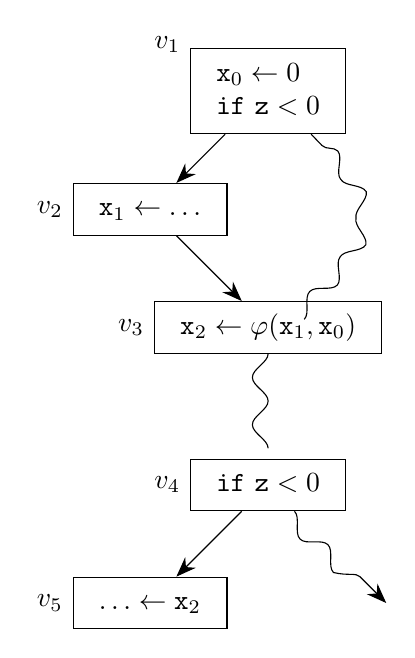
\begin{tikzpicture}
    \node[draw,label={160:{$v_1$}}] (v1) at (0,0) {\begin{tabular}{l}
            $\ttx_0\leftarrow 0$ \\
            \verb|if| $\ttz < 0$
        \end{tabular}};
    \node[draw,label={180:{$v_2$}}] (v2) at (-1.5,-1.5) {\begin{tabular}{l}
            $\ttx_1\leftarrow\ldots$
        \end{tabular}};
    \node[draw,label={180:{$v_3$}}] (v3) at (0,-3) {\begin{tabular}{l}
            $\ttx_2\leftarrow\varphi(\ttx_1,\ttx_0)$
        \end{tabular}};
    \node[draw,label={180:{$v_4$}}] (v4) at (0,-5) {\begin{tabular}{l}
            \verb|if| $\ttz<0$
        \end{tabular}};
    \node[draw,label={180:{$v_5$}}] (v5) at (-1.5,-6.5) {\begin{tabular}{l}
            $\ldots\leftarrow\ttx_2$
        \end{tabular}};
    \path[-{Stealth[scale=1.5]}] (v1) edge (v2) (v2) edge (v3) (v4) edge (v5);
    \draw[-{Stealth[scale=1.5]},
        decorate,
        decoration={
                snake, amplitude=1mm,
                segment length=6mm,
                pre length=2mm,
                post length=3mm
            }
    ] (v1) to[out=-45,in=45,looseness=1.5] (v3)
    (v3) -- (v4)
    (v4) to[out=-45,in=135] ($(v4)+(1.5,-1.5)$);
\end{tikzpicture}
\end{document}